\documentclass[a4paper,11pt]{article}

\usepackage[T1]{fontenc}
\usepackage[utf8]{inputenc}
\usepackage[czech]{babel}
\usepackage[top=3cm, left=2cm, textwidth=17cm, textheight=24cm]{geometry}
\usepackage{multirow}
\usepackage[ruled, czech, linesnumbered, noline, longend]{algorithm2e}
\usepackage{graphics}
\usepackage{pdflscape}
\usepackage{float}
\usepackage{tabularx}
\usepackage{array}


\usepackage[unicode, hidelinks]{hyperref}
\usepackage[nodayofweek]{datetime}
\usepackage[hyphenbreaks]{breakurl}
\usepackage{csquotes}
 
\begin{document}

\begin{titlepage}
    \begin{center}
        
        \Huge
        \textsc{Vysoké učení technické v~Brně}\\[0.1em]
        
        \huge
        \textsc{Fakulta~informačních technologií}
        
        \vspace*{\stretch{0.382}}
        
        \LARGE
        Modelování a simulace \\
        Elektromobilita v Brně

        \vspace*{\stretch{0.618}}
    \end{center}
    
    {\large \today \hfill Tomáš Dolák (xdolak09), Monika Zahradníková (xzahra33)}
\end{titlepage}

\newpage
\tableofcontents

\newpage
\label{firstpage}

\section{Úvod}
Jako téma našeho projektu jsme si zvolili modelování elektromobility v Brně. Elektromobilita je v posledních aktuálním trendem, 
který se v posledních letech stává stále populárnějším a je pravděpodné, že tomu bude tak i nadále. 
V rámci projektu se zaměříme na modelování elektromobily v Brně elektromobility v Brně s cílem určit zda je Brno, připraveno 
na budoucnost.\cite{simlib_cpp}

\section{Cíle projektu}
Cílem projektu je vytvořit model, který bude schopen simulovat chování elektromobilů v Brně. 
Model bude zahrnovat informace o elektromobilech, nabíjecích stanicích a o cestách, kterými 
se elektromobily v Brně pohybují. Model bude schopen simulovat chování elektromobilů v Brně 
v závislosti na různých parametrech, jako je například počet elektromobilů, počet nabíjecích 
stanic, dostupnost nabíjecích stanic, atd. Model bude sloužit k analýze a optimalizaci 
elektromobility v Brně.

\section{Rozbor tématu a použitých metod/technologií}
Pro korektní modelování elektromobility je potřeba si nejprve uvědomit, jak elektromobily fungují, 
jaké jsou jejich vlastnosti/parametry, které v modelu budou definovat transakce. Mezi hlavní aspekty,
ovlivňující chování elektromobilů, patří v prvé řadě jejich motor a akumulátor/baterie.

\subsection{Elektromotor}
U každého vozidla je nejdůležitější jeho pohon a palivo. Pro elektromobily je pohon zajištěn 
elektromotorem, který je základní součástí elektrického hnacího systému. Elektromotor přeměňuje 
elektrickou energii z baterie na mechanickou energii potřebnou pro pohyb vozidla a skládá se 
primárně ze dvou hlavních částí -- rotoru a statoru. \cite{typy_elektromotoru}

Rotor je pohyblivá část elektromotoru. Jedná se o součást, která se otáčí a přenáší mechanickou 
energii na hnací ústrojí vozidla. Pohyb rotoru je vyvolán magnetickými silami, které vznikají mezi 
ním a statorem. Rotor může být vyroben z permanentních magnetů (v motorech s permanentními magnety) 
nebo z vodivých materiálů, které reagují na elektromagnetické pole statoru (v asynchronních motorech). \cite{elektromotor}

Stator je naopak pevná část elektromotoru, která obklopuje rotor. Obsahuje sady cívek, které jsou 
napájeny elektrickým proudem z baterie. Když těmito cívkami prochází proud, vytváří elektromagnetické 
pole. Toto pole interaguje s magnetickým polem rotoru a vytváří točivý moment, který pohání rotor. \cite{elektromotor}

\begin{figure}[H]
    \centering
    \scalebox{0.25}{
        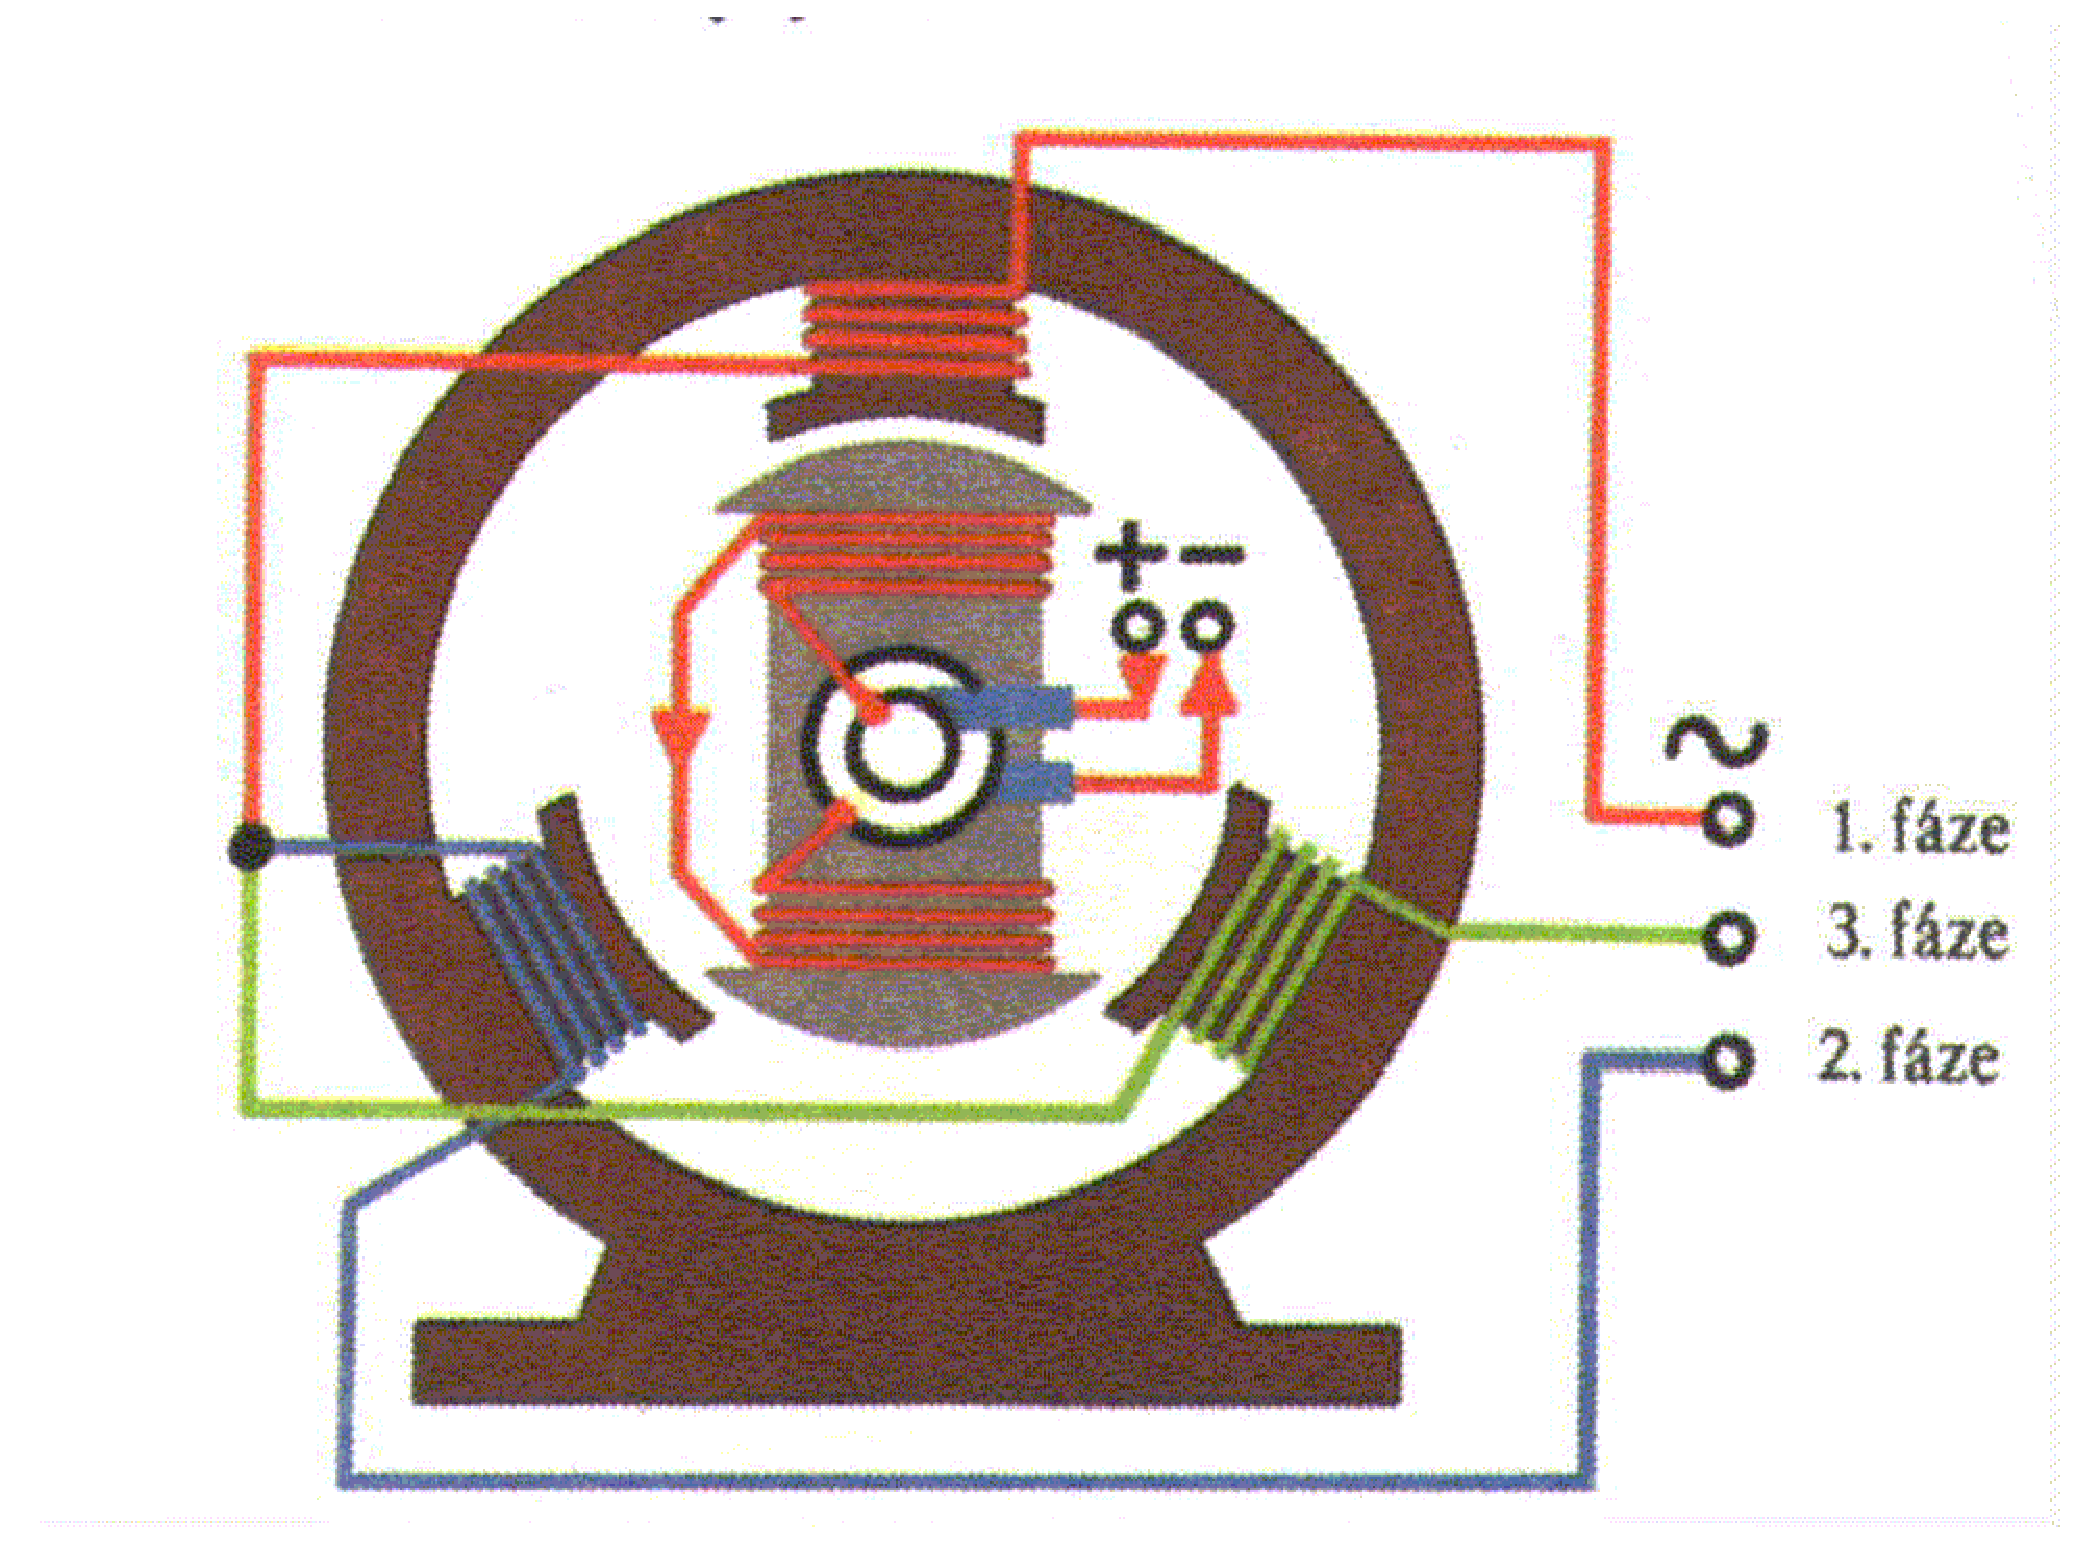
\includegraphics{synchroni-elektromotor.eps}
    }
    \caption{Schéma synchronního elektromotoru \cite{elektromotor}}
    \label{figure:synchroni-elektromotor}
\end{figure}

\subsection{Baterie}
Baterie je další důležitou součástí elektromobilu. Stejně jako existuje více typů elektromotorů, 
liší se i baterie, používané jednotlivými výrobci. V zásadě se ale jedná o lithium-iontové baterie
(varianty LIB a Li-NMC), poskytující přijatelný poměr mezi kapacitou, hmotností a prostorem, který 
zabírají.\cite{baterie_ev_wiki} Liší se však v použitelné kapacitě této baterie, které se pohybuje 
v rozmezí od 123 kWh, po 21.3 kWh na základě dat z webové stránky www.ev-database.org\cite{ev_database}, 
poskytující databázi o elektromobilech.

\subsection{Typy nabíjení}
Elektromobil, lze nabíjet hned několika způsoby, faktorů je mnoho, výkon elektrostanice, typ proudu, konektor,...
My jsme se v našem modelu rozhodli zachovat pouze podstatné parametry, které v našem případě budou mít největší 
vliv na chování elektromobilů a to nabíjecí výkon a druh proudu. Elektromobil, zde obvykle nabíjet jak 
stejnosměrným proudem, tak střídavým proudem.

\begin{figure}[H]
    \centering
    \scalebox{0.2}{
        \includegraphics{difference-between-ac-and-cd-charging-ev.eps}
    }
    \caption{Rozdíl mezi nabíjením střídavým a stejnosměrným proudem \cite{rozdil_mezi_ac_dc_nabijenim}}
    \label{figure:difference-between-ac-and-cd-charging-ev}
\end{figure}

Rozdíl ale je v jejich efektivitě, u nabíjení střídavým proudem nezáleží pouze na výkonu nabíjecí stanice, 
ale také na samotném vozidle. Baterie elektromobilu je schopna pracovat pouze se stejnosměrným proudem, 
proto je potřeba mít v elektromobilu vestavěný měnič (palubní nabíječka), který střídavý proud převede 
na stejnosměrný. Palubní nabíječka obvykle pracuje s výkonem 3,6 kW, 7,2 kW, 11 kW nebo 22 kW,
který obvykle limituje nabíjení elektromobilu, daleko víc než výkon nabíjecí stanice. \cite{nabijeni_ev}
Zato nabíjení stejnosměrným proudem je mnohem efektivnější, nemusí se měnit typ proud a nabíjení není limitováno
vůbec výkonem palubní nabíječky. Tyto nabíjecí stanice obvykle poskytují výkon 50 kW, 150 kW nebo až 350 kW.\cite{nabijeni_ev, data_brno}

U nabíjení stejnosměrným proudem se standardně cyklus nabíjení skládá ze tří fází (tzv. SoC -- State of Charge), první
fáze se pohybuje v rozmezí 0 až 20\% kapacity baterie, zde pomalu výkon narůstá, tato fáze je omezena komunikací
mezi nabíjecí stanicí a elektromobilem a také teplotou baterie. Druhá fáze začíná na 20\% až 80\% zde se na začátku
stavu dosáhne maximální výkon stanice (většínou stanice jelikož elektromobily mají zpravidla povolený větší maximální výkon
než dnešní stanice standardně nabízejí) a následně začíná pokles, tento sestupný trend nastává jak se baterie plní a
zároveň se přehřívá. Poslední fází je rozsah mezi 80\% až 100\%, zde se výkon nabíjení opět snižuje, jelikož
dochází k protekci před přebitím baterie a i chemický proces, ke kterému dochází v baterii je méně efektivní 
při vyšších úrovních nabití, což má za následek že stejný nabíjecí proud má menší dopad na zvýšení kapacity.\cite{nabijeci_krivka}

\begin{figure}[H]
    \centering
    \scalebox{0.25}{
        \includegraphics{ac-dc-charging-efficency.eps}
    }
    \caption{Efektivita AC a DC nabíjení \cite{rozdil_mezi_ac_dc_nabijenim_graf}}
    \label{figure:ac-dc-charging-efficency}
\end{figure}

U nabíjení na střídavý proud je situace jiná, tím, že je výkon primárně limitován elektromobilem -- tedy palubní nabíječkou 
(OBC - On-Board Charger), výrobce automobilu zaručuje, že baterie je schopna pracovat s určitým výkonem, který externí
nabíjecí stanice schopna poskytnout. % TODO: Dopsat!

\subsection{Elektronabíjecí stanice}

\subsubsection{Jak je na tom s elektrno stanicemi Brno?}
V Brně je celkem 102 veřejných nabíjecích stanic, vyplývající z dat z webu www.data.brno.cz\cite{data_brno},
na této stránce je i vytvořený dataset s mapou, kde jsou všechna data zaznamenána a zpřístupněna veřejnosti.
My jsme tento dataset využili a zpracovaná data, lze najít ve složce \texttt{data/} v souboru \texttt{brno\_charging\_stations.xl}.
V zásadě Brno poskytuje nabíjecí stanice s výkonem od 3.7 kW (AC) až po 108 kW (DC), a nabíjecích bodů je 
celkově 130.

% TODO: tabulka rozdeleni elektrostanic

\subsubsection{Zpracování datasetu}
Text

% TODO: popis jak jsme vyuzili dataset a jak jsme ho zpracovali

Prumerny nabijeci vykon nabijecky
\smallskip

\begin{center}
    \vspace{0.5cm} % Space before table
    \begin{tabular}{|c|c|c|c|}
        \hline
        \textbf{} & \textbf{0 - 20 [\%]} & \textbf{20 - 80 [\%]} & \textbf{80 - 100 [\%]}\\
        \hline
        12kWh AC  &  12kWh  & 12kWh & 9kWh  \\
        \hline
        22kWh AC  &  22kWh  & 22kWh & 16.5kWh  \\
        \hline
        50kWh DC  &  26kWh  & 42kWh & 17kWh    \\
        \hline
        108kWh DC &  54kWh  & 90kWh & 36.72Kwh \\
        \hline
    \end{tabular}
    \vspace{0.5cm} % Space after table
\end{center}

\begin{center}
    \vspace{0.5cm} % Space before table
    \begin{tabular}{|c|c|c|c|}
        \hline
        \textbf{} & \textbf{0 - 20 [\%]} & \textbf{20 - 80 [\%]} & \textbf{80 - 100 [\%]}\\
        \hline
        12kWh AC  &  0 -- 2.387h.  & 0 -- 5.728h. & 0 -- 3.509h.  \\
        \hline
        22kWh AC  &  0 -- 1.302h.  & 0 -- 3.096h. & 0 -- 1.914h.  \\
        \hline
        50kWh DC  &  0 -- 0.573h.  & 0 -- 1.364h. & 0 -- 0.842h.  \\
        \hline
        108kWh DC &  0 -- 0.159h.  & 0 -- 0.636h. & 0 -- 0.390h.  \\
        \hline
    \end{tabular}
    \vspace{0.5cm} % Space after table
\end{center}


\newpage
\bibliographystyle{unsrt}
\bibliography{resources}      
\end{document}